\documentclass[9pt,addpoints]{exam}
\usepackage{enumitem}
\usepackage{amsfonts,amssymb,amsmath, amsthm}
\usepackage{graphicx}
\usepackage{systeme}
\usepackage{pgf,tikz,pgfplots}
\pgfplotsset{compat=1.15}
\usepgfplotslibrary{fillbetween}
\usepackage{mathrsfs}
\usetikzlibrary{arrows}
\usetikzlibrary{calc}
\pagestyle{headandfoot}
%\firstpageheadrule
\runningheader{Current}{}{Page \thepage\ of \numpages}
\runningheadrule
\author{Aaron GK}
\usepackage{geometry}
\geometry{
	a4paper,
	total={170mm,257mm},
	left=10mm,
	right=10mm,
	bottom=5mm,
	top=5mm,
}
\firstpagefooter{}{}{}
\runningfooter{}{}{}
\begin{document}
\title{Current Electricity}
\maketitle
\section*{Current}
The flow of charges between two points in space is driven by a 
potential difference between the points. Whenever there is a net flow of charge through some region, an \textbf{electric current} is said to exist. Thus we can define current to be the net flow of charges per a given amount of time. Thus, 
$$\text{Current} = \frac{\text{Charge flow}}{\text{time taken}}$$
We use the symbol \textbf{I} to represent current. 
$$I = \frac{\varDelta Q}{\varDelta t}$$
The SI unit of current is Ampere(A). Thus, 1 Ampere is a flow of one Coulomb of charges in 1 second.
$$1 A= \frac{1 C}{1 S}$$
To understand how current flows through a conducting wire, let's look at the following cross-section of a conductor. \\
\begin{center}
	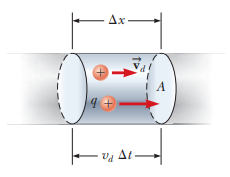
\includegraphics[scale=1]{conductor.png}
\end{center}	 
Let there be a quantity called electron density(n) which measures the number of electrons in a given volume in the conductor. The volume in the conductor above is given by the following formula:
$$V = A \varDelta x$$
The total charge in a system is the elementary charge(\textit{e}) multiplied by the number of particles carrying that charge($n_e$)
$$Q = n_e \times \textit{e}$$
We have seen above that n is the number of electrons per a given volume, thus:
$$n = \frac{n_e}{V}$$
We know that current is the flow of charges per given time:
$$I = \frac{\varDelta Q}{\varDelta t}$$
$$I = \frac{n_e \times e}{\varDelta t}$$
$$I = \frac{n \times V \times e}{\varDelta t}$$
$$I = \frac{n \times A\varDelta x \times e}{\varDelta t}$$
But, $$\frac{\varDelta x}{\varDelta t} = v \text{   - drift velocity}$$
Thus, the current becomes:
$$I = n \times A \times v\times e$$
$$I = nAve$$
Thus, the current through a conductor is affected by the electron density, the base area of the wire, the drift velocity and the elementary charge.

\section*{Sources of Electric Current}
We have seen that for current to flow, there should a be a potential difference between two points. Thus, if we have a source of a potential difference, we can have current.
\subsection*{Electrolysis}
Battery Dry Cells and other types of batteries are sources of potential difference as a result of a chemical reaction happening inside these batteries. As chemical reactions occur inside these materials, movement of charges is triggered and thus a potential difference is created. \newline
Batteries that run out of chemicals and thus run out of potential difference are called primary cells while batteries that can be recharged are called secondary cells.
\subsection*{Thermoelectric Effect}
This is the generation of potential difference as a result of temperature differences in a thermocouple. \textbf{Seebeck effect} is the EMF that develops due to temperature difference between the two ends of a thermocouple. It states that the temperature difference is directly proportional to the temperature difference between the two ends.

$$\varDelta\text{T  }\alpha\text{  }I$$

\section*{Ohm's Law}
As current flows through a conducting wire, it might face some opposition as a result of the random motion of charge carriers and the atomic interaction between them; we call this opposition to current flow the \textbf{resistance} of a wire. \newline

In a conductor, at constant temperature, the voltage is directly proportional to the current. 
\begin{center}
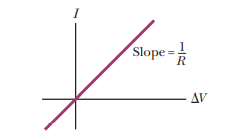
\includegraphics[scale=1]{iv_curve.png}
\end{center}
$$V\text{b  }\alpha\text{  }I$$
The constant of this proportionality is called the resistance of the wire(R).
$$V=IR$$ 
$$R=\frac{V}{I}$$
The SI unit of Resistance is called \textbf{Ohm} and we represent it with capital Omega($\varOmega$), thus:
$$1\varOmega = \frac{1 V}{1A}$$
Resistance can be affected by a number of factors.
\begin{itemize}
	\item \textbf{Temperature} - as the temperature of a conductor increases, the resistance of the conductor increases. This is because with increase in temperature, the average kinetic energy increases as well. That means, in the random motion of charge carriers, the collision increases thereby increasing the opposition to the current flow thereby \textbf{increasing resistance}.
	\item \textbf{Area} - with areal increase, however, charge carriers have wider paths to take in a wire. Thus, the opposition to the current flow decreases, thereby \textbf{decreasing resistance}.
	\item \textbf{Length} - as the length increases, the chances of collision between the charge carriers increases and therefore the opposition to current flow increase. Thus, as length increases, the \textbf{resistance also increases}.
\end{itemize}
That means, Resistance is directly proportional to temperature and length while it is inversely proportional to the area. We can mathematically describe this as:

$$R\text{  }\alpha\text{  }\frac{L}{A}$$   	
The constant of proportionality in this relationship is called the \textbf{resistivity}($\rho$) of a conductor.
$$R=\rho \frac{L}{A}$$
We can express resistivity in terms of resistance, length and area as follows.
$$\rho = \frac{RA}{L}$$
The SI unit of resistivity is $\varOmega m$. \newline \newline
Keeping the other physical quantities constant, temperature can affect the resistance in the following manner. 
$$\varDelta R\text{  }\alpha\text{  }\varDelta T $$
$$\varDelta R\text{  }\alpha\text{  }R_0 $$
Thus,
$$\varDelta R\text{  }\alpha\text{  }\varDelta T R_0$$	
The constant of proportionality for this relationship is called the temperature coefficient of resistance($\alpha$).
$$\varDelta R=\alpha\varDelta T R_0$$
We can see that the temperature coefficient of resistance of a material($\alpha$) is unique to a substance.
Since we have now found the change in resistance in terms of the initial resistance, we can find the resistance after the temperature has changed using the following relationship.
$$\varDelta R=  R- R_0$$
$$R = \varDelta R + R_0$$
$$R =\alpha\varDelta T R_0  + R_0$$
$$R =R_0(1+\alpha\varDelta T)$$
Another important concept to consider while reading topics in physics, it is imperative to note that change in temperature is the same $^0\text{C}$ and K.
$$\varDelta T_K = T_{KF} - T_{KI}$$
The change in temperature is the final temperature minus the initial temperature.
$$\varDelta T_K = (T_{CF} + 273) - (T_{CI}+273)$$
$$\varDelta T_K = T_{CF}  - T_{CI}$$
$$\varDelta T_K = \varDelta T_c$$

\textbf{Try it yourself}: Show that temperature change in Fahrenheit in terms of the change in Celsius is:
$$\varDelta T_F = \frac{9}{5}\varDelta T_C$$
\subsubsection*{Conductivity}
The conductivity of a material is how well current can pass through it. We have seen earlier that resistivity is unique to a conductor and is its ability to hinder current. Conductivity, however, is the opposite- it is a measure of how well current can pass through a wire. Mathematically, it is the reciprocal of resistivity.
$$\sigma=\frac{1}{\rho}\text{, where }\sigma\text{ is conductivity and }\rho\text{ is the resistivity.}$$

\subsection*{Deeper Dive}
There is a quantity called \textbf{current density(J)} which is a measure of the amount of current passing through a given area.
$$J = \frac{I}{A}$$
Thus, the SI unit of current density is Ampere's per square meter  $\frac{A}{m^2}$.
We have seen in unit 2 while studying electrostatics that the electric field strength is the electric force acting per a coulomb of charge. The electric field strength of a field is related to current density in the following manner.
$$J = \sigma E $$
Where E is the electric field strength and $\sigma$ is the conductivity.

\section*{Combination of Resistors}
As we have seen while studying capacitors, we usually combine circuit elements together to come up with an optimal combination of the physical quantities that we want. Resistors are no strangers to this phenomenon, and thus we can combine resistors to have an effective resistance.

\subsubsection*{Series Combination}
When resistors are connected in a manner where there is only one path for a current to flow through them, the combination is called a series combination of the resistors. In this combination, the current that is flowing through the circuit is the same through all the resistors while the voltage is the sum. \newline \newline
Look at the following combination of resistors for instance,
\begin{center}
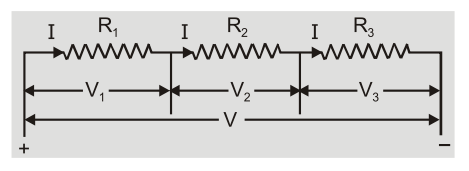
\includegraphics[scale=0.5]{series_resistors.png}	
\end{center}
We know that the voltage from the battery is the sum of the potential differences across each resistors.
$$V = V_1 + V_2 + V_3$$
We have seen according to Ohm's Law that,
$$V=IR$$
Thus, we have the following
$$IR =I_1R_1 + I_2R_2 + I_3R_3$$
We know that the current through each resistor is the same, that means
$$I = I_1 = I_2 = I_3$$
Then we plug the following into our original question.
$$IR =IR_1 + IR_2 + IR_3$$
$$IR =I(R_1 + R_2 + R_3)$$
$$R =R_1 + R_2 + R_3$$
That means, the equivalent resistance of a circuit in which all the resistors are connected in series is the sum of each resistance.
\subsubsection*{Parallel Combination}
A parallel combination means that a wire from the battery branches out and has a separate or multiple separate paths from the primary voltage wire. In such combinations, the voltage across elements that are connected in parallel is the same while the current is the sum of each current in the parallel elements.\\
Look at the following combination of resistors for instance, 
\begin{center}
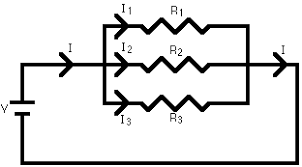
\includegraphics[scale=0.5]{parallel_resistors.png}	
\end{center}
In this case,
$$I = I_1 + I_2 + I_3$$
We know from Ohm's Law that
$$I = \frac{V}{R}$$ 
That means,
$$\frac{V}{R} = \frac{V_1}{R_1} + \frac{V_2}{R_2} +\frac{V_3}{R_3}$$	
Since
$$V = V_1 = V_2 = V_3$$
That means,
$$\frac{V}{R} = \frac{V}{R_1} + \frac{V}{R_2} +\frac{V}{R_3}$$
$$\frac{V}{R} = V(\frac{1}{R_1} + \frac{1}{R_2} +\frac{1}{R_3})$$
$$\frac{1}{R} = \frac{1}{R_1} + \frac{1}{R_2} +\frac{1}{R_3}$$
Thus, in a parallel combination of resistors, the \textbf{reciprocal} of the effective resistance is the \textbf{reciprocal} sum of each resistance.
\subsubsection*{Electric Power}
The electrical energy in a circuit, as we have seen with capacitors, is
$$E = Q \times V$$
Power, however, is the rate of energy transfer and that is
$$P= \frac{E}{t}$$
That means,
$$P = \frac{Q \times V}{t} $$
Since current is the time rate of flow of charges, we have
$$P = I\times V$$
We can also express power in terms of resistance. Ohm's Law tells us that
$$V = IR \text{ and } I=\frac{V}{R}$$
Since
$$ P = V\times I$$
$$ P = (IR)I$$
$$ P = I^2R$$
And
$$ P = V\times I$$
$$ P = V\times \frac{V}{R}$$
$$ P= \frac{V^2}{R}$$
\subsubsection*{Voltmeters and Ammeters}
\begin{itemize}
	\item An ammeter is an electric device that we use to measure current.
	\item A voltmeter is a device that can measure the potential difference across a circuit device.
\end{itemize}
As with resistors and capacitors, we have to combine a voltmeters and ammeters in a manner that is sound. \newline\newline
If we want to measure the current in a resistor, we connect the \textbf{ammeter} in series to the resistor since the current passes through the resistor and ammeter since they have a series connection.\newline
\begin{center}
	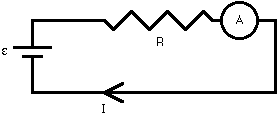
\includegraphics[scale=0.5]{ammeter.png}
\end{center}If we want to measure the potential difference across the resistor, however, we connect the terminals of the voltmeter to the ends of the resistor effectively making the connection parallel.\newline
\begin{center}
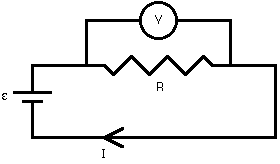
\includegraphics[scale=0.5]{voltmeter.png} 	
\end{center}
\subsection*{Electromotive Force (EMF) and Internal Resistance}
\begin{center}
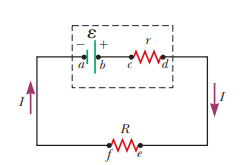
\includegraphics[scale=0.98]{emf.png}	
\end{center}
For any circuit, we usually have a battery which we use as a source of electromotive force. This is the \textbf{driving} force in a circuit that moves the charges around. \newline \newline
The EMF($\varepsilon$) of a battery is the maximum voltage a battery can provide. As with any material, even a battery has a resistance of its own. Thus, the actual voltage(V) that we measure across a battery is less than the EMF($\varepsilon$) of the battery.
$$\varepsilon > \text{V}$$ 
The small difference between the $\varepsilon$ and V is due to the resistance of the battery called \textbf{internal resistance(r)}. \\ \\
That means,
$$\varepsilon = V + \textbf{voltage dissipated due to internal resistance}$$
$$ \varepsilon = V + I r$$
If there is a load resistor(R), we can simplify the above equation as follows.
$$\varepsilon = IR + Ir$$	
$$\varepsilon = I(R + r)$$	
\end{document}